In the introduction, we left the mathematical model with an open problem: the
number of the subtour elimination constraints made infeasible the
implementation. Recalling the model we have shown before you can notice that
the variables are $\frac{n(n-1)}{2}$ and the number of constraints is
exponential because we have one subtour for almost any subset of nodes. Even if
the solution proposed in 1954 by Dantzig, Fulkerson and Johnson has been a
milestone in the history of the problem it could only solve an instance of 49
nodes. In the following years, new ways to eliminate the subtours were found
using only a linear (polynomial, in general) number of constraints. In this
chapter, we will discuss two of the most important formulations of these
compact models, build on the asymmetric version of the problem.

\section{Miller-Tucker-Zemlin}
The \emph{Miller-Tucker-Zemlin} model
\citep{miller1960integer}\citep{sawik2016note} (MTZ from now on) is defined as a
sequential formulation and it is because that the idea upon the model is to
introduce a new continuous variable $u_i$ for each node $i \in V \setminus
\{1\}$ (except the starting node). The meaning behind these $u$ variables is
to represent the order of visit of the nodes considering an optimal tour. It's
possible to define such an order because the asymmetric version of the problem
is considered. An example of such new variables is shown in figure
\ref{fig:MTZ_example}.

\begin{figure}
    \centering
    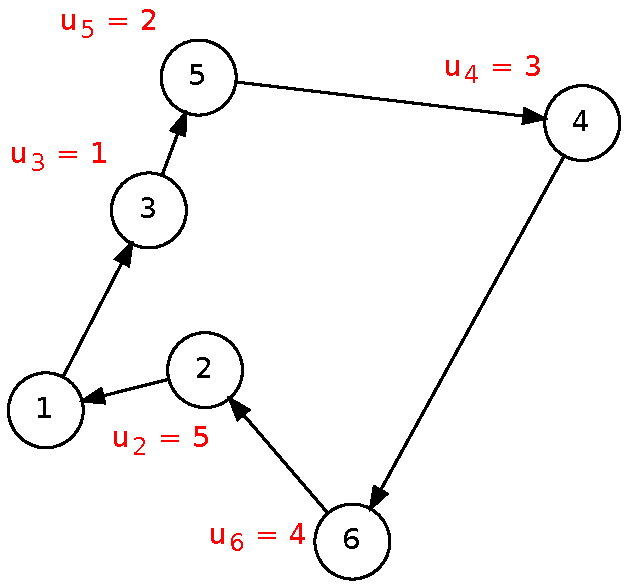
\includegraphics[width=0.43\textwidth]{figures/mtz}
    \caption[MTZ example]{Variables $u$ represent the tour visit order}
    \label{fig:MTZ_example}
\end{figure}

Given the arc $x_{ij}$ selected for the tour, the tour visit can be expressed
as $u_j \geq u_i + 1$. In symbols:


\begin{equation*} 
    \begin{array}{llr} 
        x_{ij} = 1 \implies & u_j \geq u_i + 1 & \forall i, j \in V \setminus \{1\},\ i \neq j \\
                            & u_i \in \{1, \dots\ n-1\} & \forall i \in V \setminus \{1\}
    \end{array} 
\end{equation*}

this will prevent the formation of subtours. 
The constraint is modeled as a
logic implication, but it is possible to define it also using \emph{big-M}
formulation, where the implication is dropped in favor of a modified right-hand
side that activates the constraint depending on the value of $x_{ij}$.

\begin{equation*} 
    \begin{array}{lr} 
        u_j \geq u_i + 1 \textcolor{red}{ - M (1 - x_{ij})} & \forall i, j \in V \setminus \{1\},\ i \neq j \\
    \end{array} 
\end{equation*}

that can be rewritten as

\begin{equation*} 
    \begin{array}{lr} 
        u_i - u_j + M x_{ij} \leq M - 1 & \forall i, j \in V \setminus \{1\},\ i \neq j \\
    \end{array} 
\end{equation*}

The bounds on $u$ variables remain unaltered. $M$ is supposed to be a
value large enough to trivially truly evaluate the inequality if the arc is not
selected and considering the bounds on $u$ variables, but tight enough to
prevent numerical difficulties
\footnote{\href{https://www.ibm.com/docs/en/icos/20.1.0?topic=optimization-best-practices-indicator-constraints}{https://www.ibm.com/docs/en/icos/20.1.0?topic=optimization-best-practices-indicator-constraints}}.
The smallest (and best) value for $M$ considering the formulation is $n - 1$.

\subsection{Miller-Tucker-Zemlin model}
\begin{equation*}
    \begin{array}{lrllr}
        \textrm{minimize}   & \displaystyle\sum_{(i, j) \in A} c_{ij}  x_{ij} \\
        \textrm{subject to} & \displaystyle\sum\limits_{(i, j) \in \delta^-(j)}  x_{ij} & = & 1 & \forall j \in V\\
                            & \displaystyle\sum\limits_{(i, j) \in \delta^+(i)}  x_{ij} & = & 1 & \forall i \in V\\
                            & x_{ij} & \in & \{0,1\} & \forall (i,j) \in A \\ \\
                            & u_i - u_j + (n-1) x_{ij} & \leq & n - 2 & \forall i, j \in V \setminus \{1\},\ i \neq j \\
                            & u_i & \in & \{1,\ \dots n-1\} & \forall i \in V \setminus \{1\}
    \end{array}
\end{equation*}

We have to verify that any tour in which node 1 is not present violates the
constraint and that the tour with node 1 does not. It would led to a solution
with only one complete tour. 
We first deal with a subtour of $k$ elements not passing through node 1.

\begin{theorem} 
    Given the two degree constraints, the inequalities $u_{i} -
    u_{j} + (n-1) x_{ij} \le n-2$ $\forall i,j\in V \setminus \{1\}, i\neq j$
    guarantee that the final solution contains a tour passing through node 
    $\{1\}$ and no tours not passing through it. 
\end{theorem}

\begin{proof}
    First, prove that for any tour that not contains the starting node at least
    one of the inequalities is violated by a pair of nodes of the tour. To show
    that it is enough to sum all the constraints relative to the selected arcs.
    All u variables are summed and subtracted once. Hence the sum of the $k$
    (number of nodes in the tour) constraints will end up in an impossible
    inequality $k(n - 1) \leq k(n - 2)$. Since we know that given the degree
    constraints the solution does not contain an open path and we just saw that
    there are no tours that do not pass through the source node, it is
    sufficient to show that a tour passing through 1 can exist to prove that
    the solution returns a Hamiltonian circuit. To show that it is enough to
    verify if single constraints are violated both in case arcs are selected or
    not. For $x_{ij} = 0$ it is straightforward because $u_i - u_j \leq n - 2$
    since $u_i \leq n - 1$ and $u_j \geq 1$. Being u position variable we can
    define their value as the discrete-time $t$ in which they are visited. So
    assuming $x_{ij} = 1$ the node $i$ is visited immediately before than $j$
    so if $u_i = t$ then we can assume $u_j = t + 1$. In this way constraint is
    satisfied since $u_i - u_j + n - 1 \leq n - 2 \implies t - (t + 1) + n - 1
    \leq n - 2$ that is valid because $t - (t + 1) + n - 1 = -1 + n - 1 = n -
    2$.
\end{proof}

\subsection{CPLEX implementations}
MTZ implementation using CPLEX can be done using different techniques. Besides
the straightforward implementation of the degree constraints, MTZ's subtour
elimination constraints can be implemented in different ways. \\ One of CPLEX's
features are \emph{indicator
constraints}\footnote{\href{https://www.ibm.com/docs/en/icos/12.9.0?topic=optimization-what-is-indicator-constraint}{https://www.ibm.com/docs/en/icos/12.9.0?topic=optimization-what-is-indicator-constraint}},
a way to activate or not a certain constraint depending on the value of a
control, binary variable. Internally this is implemented with big-M technique or
through local activation of that constraint in a certain node during
branching, while that variable is fixed. This is the perfect scenario for the
first version of MTZ SECs we presented. \\ 
The other way, the one we presented in the model, uses big-M formulation, which
implementation is straightforward. We will refer to this as the \emph{static}
model. \\
Another possibility is using \emph{lazy constraints}
\footnote{\href{https://www.ibm.com/docs/en/icos/12.9.0?topic=pools-what-are-user-cuts-lazy-constraints}{https://www.ibm.com/docs/en/icos/12.9.0?topic=pools-what-are-user-cuts-lazy-constraints}}
, a type of constraints that are not immediately added to the model, but
activated once they are necessary. The idea behind this is to specify as lazy
some constraints that are unlikely to be violated, keeping the model thinner.
Again, a perfect scenario for our big-M SECs. We will refer to this as the
\emph{lazy} model. They have some limitations, the most notable is that a lazy
constraint cannot have indicator constraints, so we cannot mix the two
implementations. 

\begin{claim}
    The best implementation is the one that takes advantage of lazy constraints.
\end{claim}

\begin{figure}
    \centering
    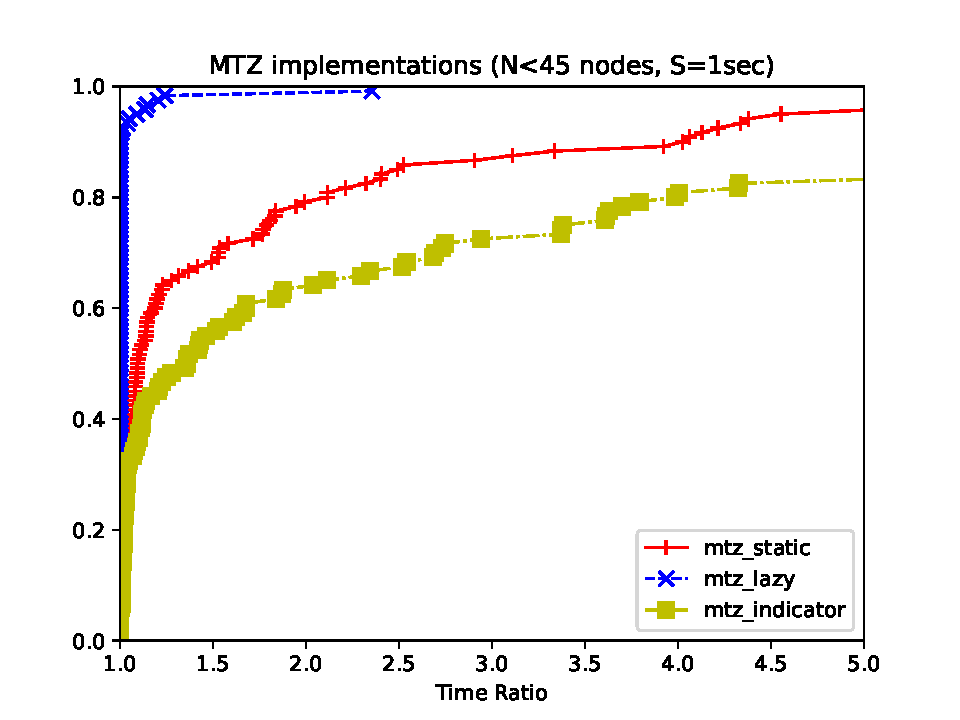
\includegraphics[width=0.8\textwidth]{figures/mtz_comp1.pdf}
    \caption{MTZ implementations comparison}
\end{figure}

The graph is representing the result of geometric-mean profiler
\citep{dolan2002benchmarking}. A total of 120 instances are tested, 30 of which
are around 45 nodes (that will ensure a $<10$ min execution time). More on
testing setup and parameters settings in appendix \ref{appendix:testenv}. \\

The result of the benchmark is pretty clear: the model implemented through lazy
constraints is faster than the other two. We can also assert that the static
model is faster than the one which uses indicator constraints.\\
Since the results allow us to and bearing in mind that correlation does not
imply causality, we can carefully assert that the smallness of the model makes
it faster. This is true if lots of constraints are not violated (then not added to the
model), while on the static all of the constraints are present at starting time.
This is also true considering the static model versus the one with indicator
constraints, which is a comparison between formulations. In fact, after an
analysis of CPLEX logs, it is possible to notice that the presolve didn't reduce
the model size with indicators, which has always more rows and more columns (in
general, more non-zeroes) than the static model. 

\begin{table}[h]
    \begin{tabular}{rl}
    \begin{tabular}[c]{@{}r@{}}Static\\ log\end{tabular}    & \begin{tabular}[c]{@{}l@{}}\footnotesize \texttt{Reduced MIP has 977 rows, 675 columns, and 3750 nonzeros.}\\ \footnotesize \texttt{Reduced MIP has 650 binaries, 25 generals, 0 SOSs, and 0 indicators.}\\ \footnotesize \texttt{...}\end{tabular} \\
    \begin{tabular}[c]{@{}r@{}}Indicator\\ log\end{tabular} & \begin{tabular}[c]{@{}l@{}}\footnotesize \texttt{Reduced MIP has 1277 rows, 975 columns, and 4050 nonzeros}.\\ \footnotesize \texttt{Reduced MIP has 650 binaries, 25 generals, 0 SOSs, and 600 indicators.}\\ \footnotesize \texttt{...}\end{tabular}                          
    \end{tabular}
    \caption[MTZ size comparison on indicator versus static model]{\centering Model size for toy example of 26 nodes. There are $300 =
    \frac{600}{2} = \frac12 2 {25 \choose 2}$ non-zeroes, rows and columns with respect to the static model}

\end{table}

In fact, for all three model sizes (rows, cols and non-zeroes) the indicator has
exactly half of the number of SECs in addition to the others. This is true for
rows and non-zeroes, while for columns, the number of variable in the static model
plus half of the number of SECs is reported in the model size section, while in
the section that exploits the nature of the variables, all of the variables in
the static one are reported, in addition to others marked as \emph{indicators}
(equal to the number of SECs). Keeping in mind that the number of SECs is $2 \cdot
{ n \choose 2} = 2 \cdot \frac{n (n - 1)}{2} \in \mathcal{O}(n^2)$, this result
cannot be ignored. Another important fact to analyze is that the presolve on the
lazy model worked really well: it drastically reduced the number of rows,
probably the key to the success of this formulation.\\

Considering how the indicator constraints are well sold on CPLEX
guidelines\footnote{\href{https://www.ibm.com/support/pages/node/397209}{https://www.ibm.com/support/pages/node/397209}},
the results are kinda surprising. But the guidelines state also that a big-M
formulation should be avoided when M is much larger than any other coefficient
and when the model does not suffer from big-M side effects (numerical issues,
mainly), that is not our case. We precisely choose $M$ and set the
parameter \texttt{CPX\_PARAM\_EPINT} to ensure general correctness. We suppose
that those advice on indicator constraints are given to prevent a poor choice
of $M$ and, consequently, a hard time debugging numerical issues, which can be
difficult to exploits.

\subsection{Speeding up the model}
The model we presented is correct, in the sense that solves the problem for a
reasonable amount of time up to a certain number of nodes. The performance of
the model, however, can be improved by adding some constraints that tight the LP
relaxation during branching. The constraints we're up to adding are SECs from
Dantzig, Fulkerson and Johnson formulation, restricted to a certain size of
subsets. The problem with that formulation is that the total number of
constraint is exponential in $n$, but the idea is to add only those constraints
that involve subsets of nodes of size 2 or at most 3.\\

We will refer as \emph{SECs of degreee 2} this constraints:

\begin{equation*} 
    \begin{array}{lr} 
        x_{ij} + x_{ji} \leq 1 & \forall i, j \in V,\ i \neq j
    \end{array} 
\end{equation*}

and as \emph{SECs of degreee 3}:

\begin{equation*} 
    \begin{array}{lr} 
        x_{ij} + x_{jk} + x_{ki} \leq 2 & \forall i, j, k \in V,\ i \neq j \neq k
    \end{array} 
\end{equation*}

This will prevent subtours of size 2 and size 3 to form. We have to keep in mind
that the total number of constraints added is not that negligible: for degree 2
SECs they are ${n \choose 2} \in \mathcal{O}(n^2)$ while for degree 3 they are
$2 \cdot {n \choose 3} \in \mathcal{O}(n^3)$. Note that for degree 3, we have to
consider both circular paths due to asymmetry (for example, considering node 2,
5 and 8, we have to add both $x_{25} + x_{58} + x_{85} \leq 2$ and $x_{28} +
x_{85} + x_{52} \leq 2$). Clearly, does not exist such degree 1 SECs because
self-loops are not allowed in the model.

The idea is to add only a small amount of constraint so the model is still
compact but powerful enough to speed up the branching process. We have to find a
trade-off for this. We can consider degree-2 constraints as a correction of the
asymmetric model with respect to the symmetric one: because of asymmetry, we
have double the number of variables, because an edge is converted in two arcs.
A degree-2 constraint for a couple of arcs means that if one of them is fixed,
also the other one had to be fixed, so we don't have freedom of choice on the
other one, exactly as the symmetric version (because there's only one edge!).
The ovehead is to have twice the variables and specialized constraints to manage
this behavior.

\begin{claim} 
    The solve time for MTZ model can be improved including deegree-2 subtour
    elimination constraints. 
\end{claim}

\begin{figure}[h]
    \centering
    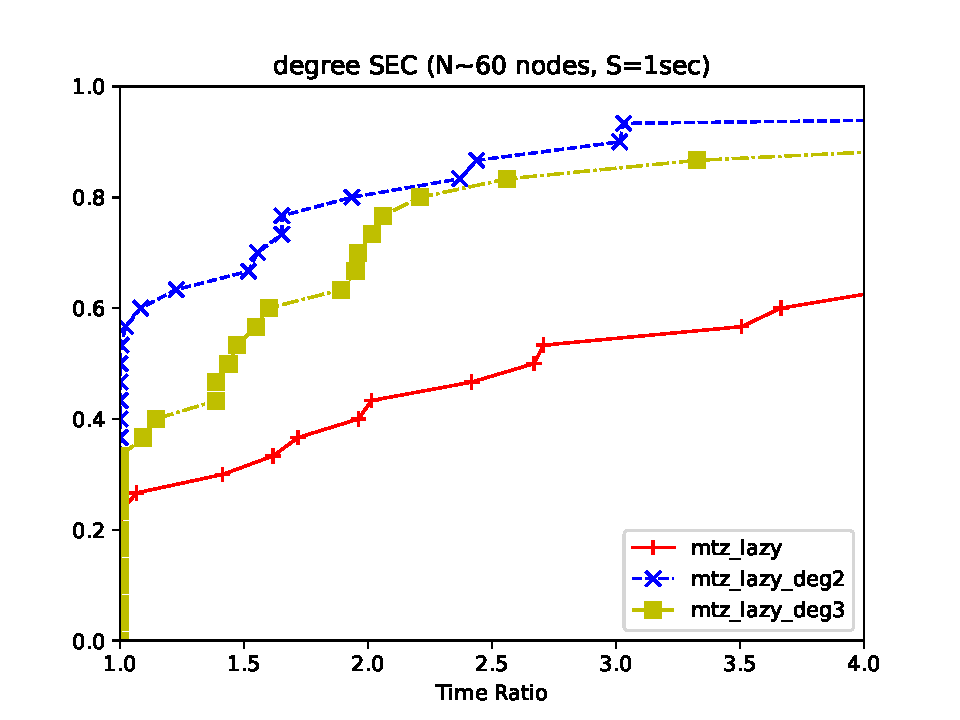
\includegraphics[width=0.8\textwidth]{figures/mtz_comp2.pdf}
    \caption{MTZ degree SECs comparison}
\end{figure}

The comparison is done on lazy implementation (because of it's superior with
respect to the others) so the number of nodes for istance can be increased to
avoid any bias: 30 istances of ~60 nodes are tested.\\

The graph shows the superiority of degree 2 SECs model with respect to a basic
implementation and to degre 3 SECs model (which includes both constraints of
degree 2 and 3). This is probably due to the number of constraints added that,
despite being lazy, they're too much considering the degree 3 model. As
we could expect, the degree 3 model works pretty well when the model is small
or easy to solve, because the total number of constraints added is not so
different than the degree 2 model. Considering that the goal is to solve
efficiently hard problems, this information is not that interesting.

\subparagraph{Note:} claim 1 was produced considering adding all the degree
2 Danzing's subtour elimination constraints. Overall, we can consider the big-M
formulation with degree 2 SECs and implemented using lazy constraints as the
winner over all possible MTZ formulations and implementations.




\section{Gavish and Graves}
In 1978 Gavish and Graves \citep{gavish1978travelling}\citep{orman2006survey}
proposed an alternative solution based on a flow idea. This method introduces a
variable $y_{ij}$ for each arc $(i,j) \in A,\ (i\neq j)$, which represents the
\emph{quantity of flow} in the arc. The source of the flow is node 1, and its
destination after visiting the graph. Starting at its maximum capacity ($n -
1$) the flow loses one unit each time it visits a node, returning to node 1
with no flow at all. Figure \ref{fig:GG_example} shows the idea in a toy
example.

\begin{figure}[h]
    \centering
    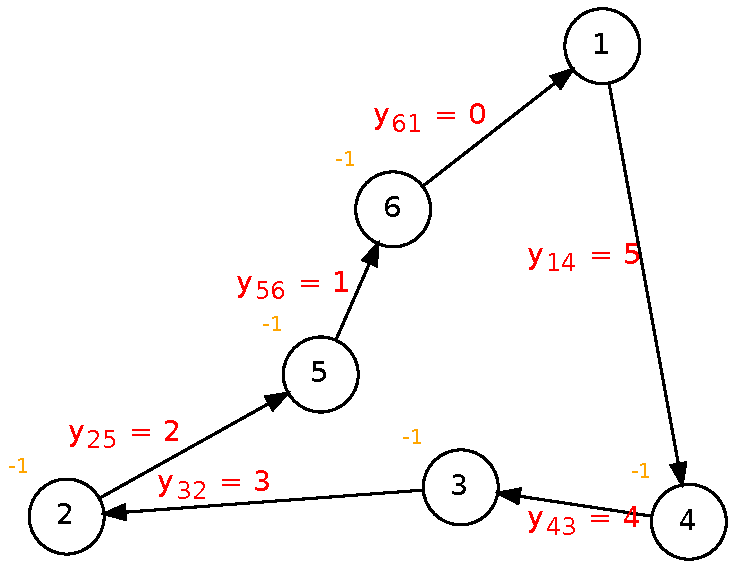
\includegraphics[width=0.43\textwidth]{figures/gg}
    \caption[GG example]{Variables $y$ represent flow quantity}
    \label{fig:GG_example}
\end{figure}

First of all, we have to model the flow. We have to model the flow at the
beginning, as well at the end, and its behavior during the visit.
Respectively, they are modeled with

\begin{equation*} 
    \begin{array}{rrlr} 
        y_{1j} & = & (n - 1) x_{1j} & \forall j \in V \setminus \{1\} \\
        y_{i1} & = & 0 &\forall j \in V \setminus \{1\} \\
        \underbrace{\displaystyle\sum\limits_{i = 1, i \neq h}^n y_{ih}}_{in-flow\ node\ h} & = & \underbrace{\displaystyle\sum\limits_{j = 1, j \neq h}^n y_{hj}}_{out-flow\ node\ h} + 1 & \forall h \in V \setminus \{1\}\\
    \end{array} 
\end{equation*}

We will refer to them as \emph{flow-model constraints}. The first one model the
out flow from node 1, which has to be set at its maximum capacity, $n - 1$.
Only one of the $x_{1j},\ j \in V \setminus \{1\}$ will be set to one so, for
that arc, the flow will be $n - 1$.\\ The second one model the in flow at node
1, which is zero, because we are supposing that during the visit of the remain
$n - 1$ nodes, the flow will decrease to zero. Notice that we can model this
constraint imposing a different upper bound to those variables: these
constraints will be dropped from the model during implementation.\\ The third
one model the leaking of one flow quantity during each visit that not involves
node 1.\\
The last thing to do is to link the flow variables to the arc selection
variables, so if an arc is selected, the flow is free to pass through it. We
can model this imposing different upper bound on flow capacity for that arc:

\begin{equation*} 
    \begin{array}{rlrr} 
        x_{ij} = 0 \implies & y_{ij} = 0 & \forall i, j \in V \setminus \{1\},\ i \neq j \\
        x_{ij} = 1 \implies & y_{ij} = n - 2 & \forall i, j \in V \setminus \{1\},\ i \neq j \\
    \end{array} 
\end{equation*}

this logical implication can be modeled as

\begin{equation*} 
    \begin{array}{rrlr} 
        y_{ij} & \leq & (n - 2) x_{ij} & \forall i, j \in V \setminus \{1\},\ i \neq j \\
    \end{array} 
\end{equation*}

We will refer to them as \emph{linking constraints}. It is possible to notice
that the in/out flow from node 1 are a special case of this constraint, in
fact, this one imposes an $n - 2$ upper bound on the value of $y_{ij}$ because
that case is already managed, and the bound can be made tighter.\\
The bound on the variables are simply

\begin{equation*} 
    \begin{array}{rrlr} 
        y_{ij} & \in & \{0,\ \dots n-1\} & \forall i,j \in V,\ i \neq j
    \end{array} 
\end{equation*}

this works in general, but on the implementation side, the bounds can be
restricted at $n - 2$ for all nodes different from 1 and to $0$ for the in-flow
variable at node 1, as previously mentioned. It's interesting to note that the 
variables are not necessarly integers, but providing such information to the
solver is always a good practice.\\ 
Since this formulation was presented in class, we will refer to
it as \emph{lecture model}, which is summarised below:

\subsection{Gavish-Graves model, lecture}
\begin{equation*}
    \begin{array}{lrllr}
        \textrm{minimize}   & \displaystyle\sum_{(i, j) \in A} c_{ij}  x_{ij} \\
        \textrm{subject to} & \displaystyle\sum\limits_{(i, j) \in \delta^-(j)}  x_{ij} & = & 1 & \forall j \in V\\
                            & \displaystyle\sum\limits_{(i, j) \in \delta^+(i)}  x_{ij} & = & 1 & \forall i \in V\\
                            & x_{ij} & \in & \{0,1\} & \forall (i,j) \in A \\ \\
                            & \displaystyle\sum\limits_{i = 1, i \neq h}^n y_{ih} & = & \displaystyle\sum\limits_{j = 1, j \neq h}^n y_{hj} + 1 & \forall h \in V \setminus \{1\}\\
                            & y_{1j} & = & (n - 1) x_{1j} & \forall j \in V \setminus \{1\} \\
                            & y_{i1} & = & 0 & \forall j \in V \setminus \{1\} \\
                            & y_{ij} & \leq & (n - 2) x_{ij} & \forall i, j \in V \setminus \{1\},\ i \neq j \\
                            & y_{ij} & \in & \{0,\ \dots n-1\} & \forall i,j \in V,\ i \neq j
    \end{array}
\end{equation*}

Even if this model is correct, it is possible to modify it while keeping
correctness. The in-flow contraints for node 1 are implicitly satisfied
considering the initial value of the flow and the fact that the flow loses one
quantity for each visit (modeled by the flow control constraints). Anyway, this
is no big deal considering that those constraints were implemented as variable
bounds.\\ The out flow constraints from node 1 can be merged in this one:

\begin{equation*} 
    \begin{array}{rrlr} 
        \displaystyle\sum\limits_{j = 1, j \neq 1}^n y_{1j} & = & n - 1 & \\
    \end{array} 
\end{equation*}

\newpage
Clearly, just one element of the sum will be equal to $n - 1$: considering the
flow loss, lenght of tour and variable bounds, the flow has to start with that
value.\\ 
We still need to link the selection of an arc starting from node 1 to
the full capacity on that arc, made possible by 

\begin{equation*} 
    \begin{array}{rrlr} 
        y_{1j} & \leq & (n - 1) x_{1j} & \forall j \in V \setminus \{1\} \\
    \end{array} 
\end{equation*}

which can be seen as a specialized case of linking constraints for node 1. The
remaining linking constraints, as well as flow-model constaints, remains
unaltered.
Since this model is the most frequent in literature, we will refer to it as
\emph{literature model}, which is summarised below:

\subsection{Gavish-Graves model, literature}
\begin{equation*}
    \begin{array}{lrllr}
        \textrm{minimize}   & \displaystyle\sum_{(i, j) \in A} c_{ij}  x_{ij} \\
        \textrm{subject to} & \displaystyle\sum\limits_{(i, j) \in \delta^-(j)}  x_{ij} & = & 1 & \forall j \in V\\
                            & \displaystyle\sum\limits_{(i, j) \in \delta^+(i)}  x_{ij} & = & 1 & \forall i \in V\\
                            & x_{ij} & \in & \{0,1\} & \forall (i,j) \in A \\ \\
                            & \displaystyle\sum\limits_{i = 1, i \neq h}^n y_{ih} & = & \displaystyle\sum\limits_{j = 1, j \neq h}^n y_{hj} + 1 & \forall h \in V \setminus \{1\}\\
                            & \displaystyle\sum\limits_{j = 1, j \neq 1}^n y_{1j} & = & n - 1 & \\
                            & y_{ij} & \leq & (n - 2) x_{ij} & \forall i, j \in V \setminus \{1\},\ i \neq j \wedge i \neq 1 \\
                            & y_{1j} & \leq & (n - 1) x_{1j} & \forall j \in V \setminus \{1\} \\
                            & y_{ij} & \in & \{0,\ \dots n-1\} & \forall i,j \in V, i \neq j
    \end{array}
\end{equation*}

\subsection{CPLEX implementations}
Both formulation allows an implementation that uses lazy constraints, so
everything will be tested. The model, anyway, it's different from MTZ by the
number of variables, which is $\mathcal{O}(n^2)$. If we exclude
SECs of degree 2, the model is bigger than MTZ, but still compact.

\begin{claim} 
    The best combination of formulation and implementation is the literature
    model implemented through static constraints. 
\end{claim}

\begin{figure}[h]
    \centering
    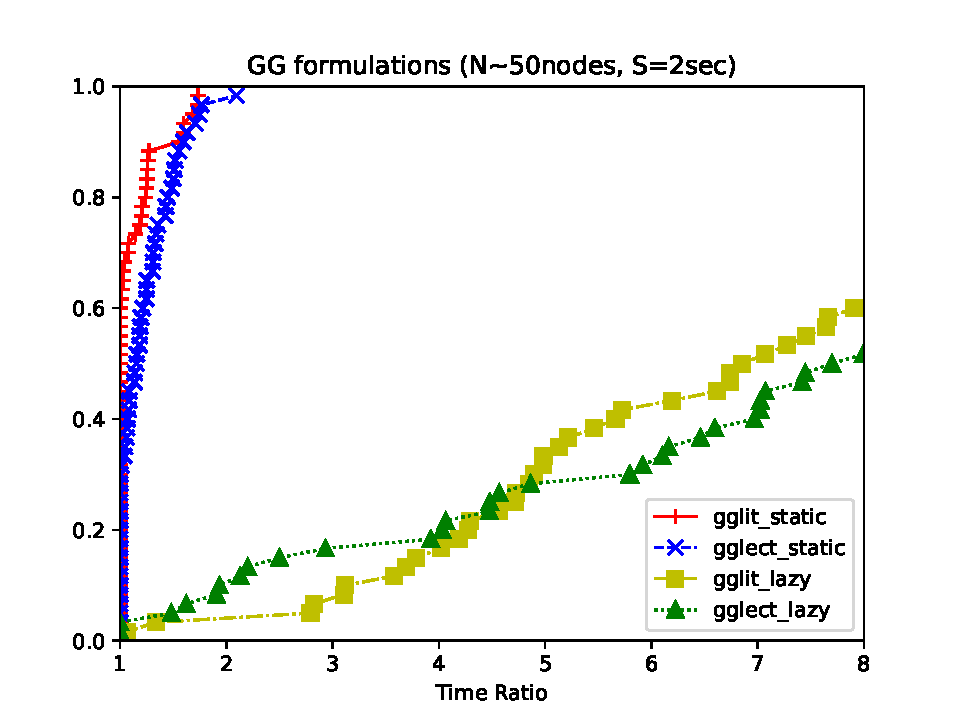
\includegraphics[width=0.8\textwidth]{figures/gg_comp1}
    \caption{GG formulations and implementations comparison}
\end{figure}

The comparison is done considering 60 instances of around 50 nodes each. It's
clear that the static implementation is better than the lazy one. Recall that
the main idea behind lazy constraints is to add them only when needed, keeping
the model small for relaxations. They are supposed to be violated very few
times, but this is not the case. The GG SECs models a behavior of lots of
variables ($\mathcal{O}(n^2)$), so it's expected that will be a lot of
constraints violated. We tested the number of constraint violation (during whole
execution) by running the lazy implementations of MTZ and GG (both formulations)
on a total of 25 instances (5 of which composed of 10 ,20, 30, 40 and 50
nodes).

\begin{figure}[h]
    \centering
    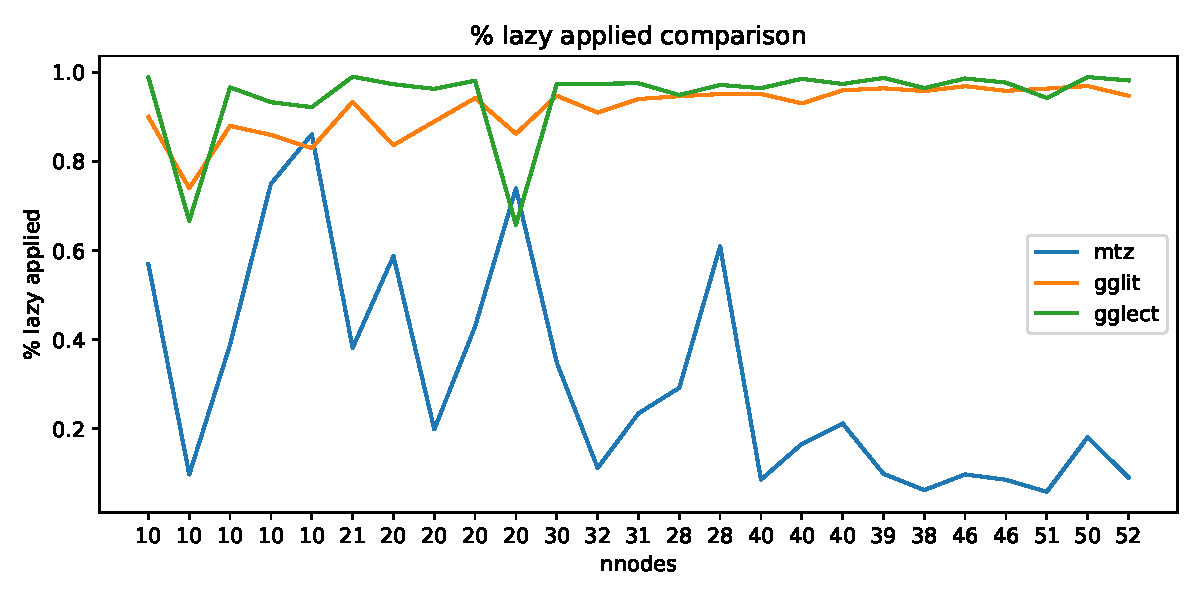
\includegraphics[width=0.78\textwidth]{figures/perc_lazy}
    \caption{Percentage of lazy violations for each model}
\end{figure}

While keeping in mind that the number of constraints is quadratic in number of
nodes, we can observe that the number of lazy violations in MTZ (blue line) is
decreasing (and independent in the number of nodes) so, roughly, constant in
absolute values, while in both formulation of GG  (orange and green lines),
almost all constraints are violated. That makes the implementation through lazy
constraints ideal for MTZ and costrly for GG, because of model reshapes during
executions.\\

Both static models are quite good, with the literature formulation that performs
slightly better that the one presented in class.


One may ask if the Dantzig's SECs for degree 2 that worked beautifully in the MTZ
model could also help here.

\begin{claim} 
    The solve time for GG model can be improved including deegree-2 subtour
    elimination constraints.
\end{claim}

We tested the best model in the previous comparison, the literature formulation
with static constraint, statically adding the additional SECs. We tested 30
instances of 80 nodes each.

\begin{figure}[h]
    \centering
    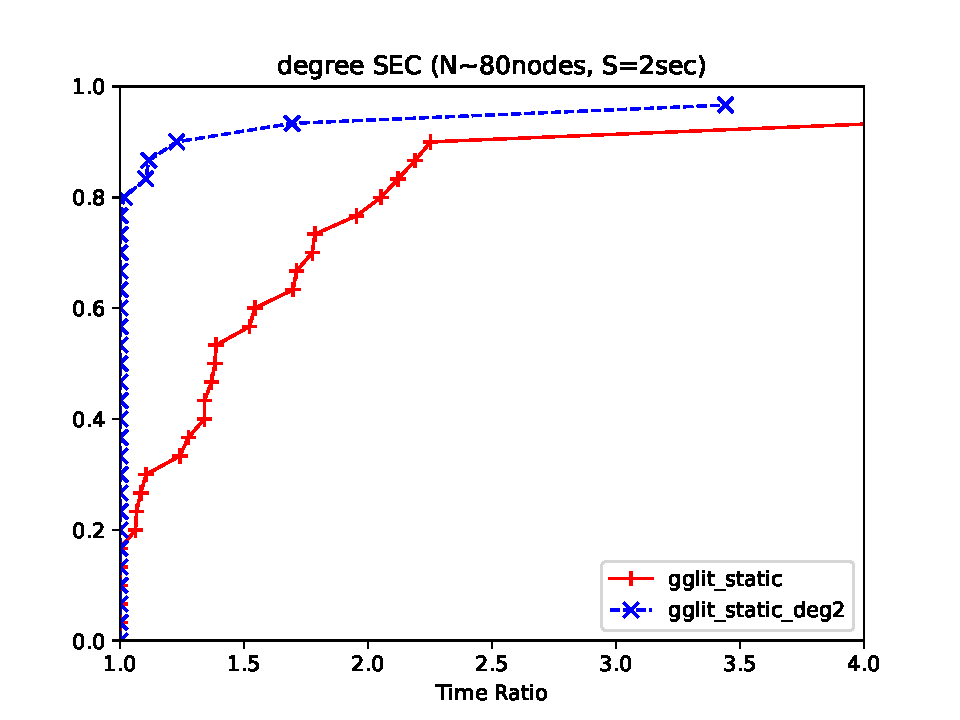
\includegraphics[width=0.8\textwidth]{figures/gg_comp2}
    \caption{GG degree SECs comparison}
\end{figure}

The answer is positive, those constaints are helpful also here. \\ 

The static implementation of the literature formulation with degree-2 SECs
is the winener among all possible formulations and implementations.

\section{Compact models comparison}
Finally, we tested MTZ agains GG, considering for both of them the optimal
formulation / implementation on a test bed of 30 instances of 80 nodes.

\begin{claim} 
    GG is a better compact model formulation of TSP compared with MTZ.
\end{claim}

\begin{figure}[h]
    \centering
    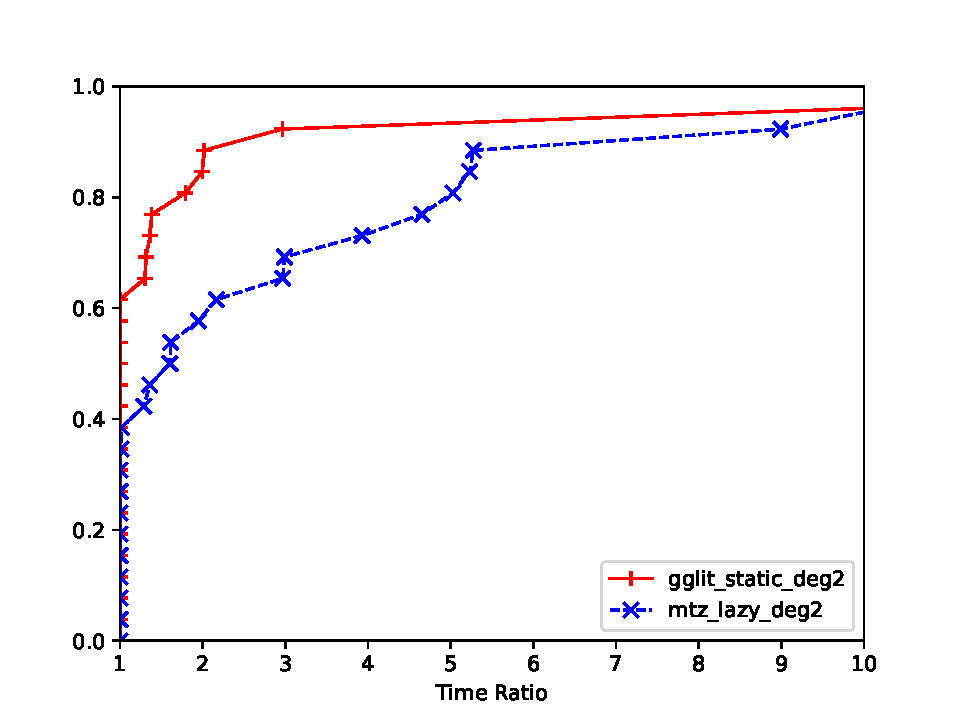
\includegraphics[width=0.8\textwidth]{figures/compact_final}
    \caption{Compact models comparison}
\end{figure}

We can decree the Gavish and Graves as the best compact model for euclidean TSP.
It's nice to notice that, give a fixed time limit, the number of nodes solved to
optimality in that timelimit act as a benchmark for the performance of the
methods and approaches to TSP. In this case, considering our setup, 80 nodes is
the maximum amount that can be solved by limiting the computation to 10 minutes.
It's also important to check each time that the solutions obtained are optimal,
in the sense that if one of the two methods reaches time limit, the beast
feasible solution obtained during branch-and-cut is obtained, but there's a loss
of sense to compare it with the other solution produced by the other method. In
our tests, we will ensure that all this details are taken into consideraiton.
